% Active Matter lab (Lab C) -- letter, single-column layout.
% Compile with:  pdflatex main && bibtex main && pdflatex main && pdflatex main     (or upload the folder to Overleaf)
% Everything marked \todo{...} (red in the PDF) still needs your input -- search for "TODO" to find them.
\documentclass[11pt]{article}

\usepackage[a4paper,margin=2.2cm]{geometry}
\usepackage{graphicx}
\usepackage{amsmath,amssymb,bm}
\usepackage{xcolor}
\usepackage[numbers,sort&compress]{natbib}
\usepackage[colorlinks=true,linkcolor=blue!50!black,citecolor=blue!50!black,urlcolor=blue!50!black]{hyperref}
\usepackage{setspace}
\setlength{\parskip}{0.3em}
\setlength{\parindent}{1.2em}
\bibliographystyle{unsrtnat}

\newcommand{\todo}[1]{\textcolor{red}{\textbf{[TODO: #1]}}}
\newcommand{\ee}{\hat{\mathbf e}}
\newcommand{\rr}{\mathbf r}

\title{\vspace{-1.5em}Active Matter - Lab C}

\author{Yael Yaari \and Netta Kaplan\\[0.3em]}

\date{November 15, 2026}

\begin{document}

\maketitle

\begin{abstract}
We show that the persistent motion of vibration-driven robots (Hexbugs) is enough to make their bath a rectifier: the shape of an object immersed in it, not the bugs, sets the direction in which the object is driven.
Gears whose teeth have opposite orientation rotate in opposite senses at about $25$ to $40\,^\circ$/s, each in a single sense in 49 of 53 windows of $8\,$s, with no resolvable dependence on the number of bugs between 10 and 17.
A mirror-symmetric straight rod has no net motion along its axis, as symmetry requires, whereas an L-shaped rod is about $50\%$ faster but, within our statistics, does not select a direction along its axis.
The single-bug motion behind this is ballistic for about $2.6\,$s, as for an active Brownian particle; at longer times a weak, steady turning bias of the bug replaces the expected diffusion by a plateau of the mean square displacement followed by superdiffusion.
\todo{one sentence on the number-fluctuation result of the flocking experiment}
\end{abstract}

Active matter is made of units that convert energy into self-propulsion, from swimming bacteria and self-propelled colloids to animal groups and robots~\cite{Marchetti2013,Bechinger2016,VicsekZafeiris2012}.
Because every unit is driven, these systems are out of equilibrium and display phenomena without passive counterparts: self-propelled particles undergo a transition to collective motion~\cite{Vicsek1995}, flocks can sustain long-range order in two dimensions in spite of the equilibrium prohibition~\cite{TonerTu1995}, birds in a flock interact with a fixed number of neighbours rather than with all neighbours within a fixed distance~\cite{Ballerini2008}, and repulsive particles with no attraction cluster and phase-separate~\cite{Buttinoni2013,CatesTailleur2015}.

Persistent motion also makes active particles exquisitely sensitive to geometry: they accumulate at walls and obstacles~\cite{Bechinger2016}, and asymmetric shapes rectify their otherwise random motion.
A wall of funnels concentrates swimming bacteria on one side of a chamber~\cite{Galajda2007}, a result that simulations trace to the ballistic part of the trajectories~\cite{Wan2008}; and asymmetric micro-gears rotate spontaneously in a bath of bacteria~\cite{Angelani2009,DiLeonardo2010,Sokolov2010}, whereas symmetric gears do not~\cite{DiLeonardo2010}.

At the level of a single particle, active motion is directed at short times and becomes a random walk with enhanced diffusion at long times~\cite{Howse2007,tenHagen2011}.
Hexbugs reproduce this phenomenology at the scale of centimetres: they perform active Brownian motion, with a chiral correction from the motor, and can move and rotate passive objects~\cite{Balda2022}; vibration-driven robots also show an inertial delay between their orientation and their velocity~\cite{Scholz2018}.
A particle whose propulsion is not aligned with a symmetry axis of its body swims in circles~\cite{Kummel2013}, which is the form such a correction takes.

In this letter we show that a bath of Hexbugs turns its persistence into directed motion of the objects it pushes, with the direction set by the symmetry of the object.
We first show that a single bug moves ballistically for about $2.6\,$s, as an active Brownian particle does, and that the departure from the expected diffusion at longer times, a plateau and then superdiffusion, is accounted for by a weak steady turning bias of the bug together with a slow drift.
We then show that gears with opposite tooth orientation turn in opposite senses, each steadily, and that the rate is not resolvably changed between 10 and 17 bugs.
Finally, we show that a straight rod, which is mirror symmetric, has no net motion along its axis, while an L-shaped rod moves faster but, with the data we have, no preferred direction along its axis can be established.
\todo{sentence on the flocking / number-fluctuation result}

\bigskip
\noindent Hexbugs ($5\,$cm long) were filmed from above at 30 frames/s inside custom arenas \todo{arena shapes and sizes in cm; px/cm calibration; camera height}.
A single bug was located in every frame with a circular Hough transform; when several circles were detected, those further than $300\,\Delta t+20\,$px from the last accepted position were discarded and the remaining centres, if all within 30 px of each other, were averaged.
The gears and rods carry painted markers (two orange or one green and one orange dot on the gears, one green dot on the rods) that were located by colour thresholding.
Frames in which a hand was in view (skin-coloured pixels) were excluded.
Lengths are given in pixels (px) \todo{convert to cm once the calibration is known}.

We start with the single bug.
The simplest description of a self-propelled particle whose heading is randomised by noise is the active Brownian particle (ABP) model, for which the speed $v_0$ is constant, the heading $\theta$ diffuses with rotational diffusion coefficient $D_r$, and translational diffusion is negligible for a macroscopic robot~\cite{Balda2022}.
The Hexbug's body is not exactly left--right symmetric, and a pure ABP cannot describe our data without two small corrections: a mean rotation rate $\Omega$ of the heading (a chiral ABP~\cite{Kummel2013}) and a constant drift $\mathbf V$ of the orbit centre,
\begin{align}
  \dot{\rr} &= v_0\,\ee(\theta)+\mathbf V, \label{eq:r}\\
  \dot{\theta} &= \Omega+\sqrt{2D_r}\,\xi(t), \label{eq:th}
\end{align}
where $\ee(\theta)=(\cos\theta,\sin\theta)$ and $\xi$ is unit white noise.
For $\Omega=0$ and $\mathbf V=0$ this is the standard ABP: the heading is forgotten after $\tau_r\simeq1/D_r$, motion is ballistic for $t\ll\tau_r$ and diffusive with $D_\mathrm{eff}=v_0^2/2D_r$ for $t\gg\tau_r$.
For $\Omega\neq0$ the heading correlation becomes $\langle\ee(t)\!\cdot\!\ee(0)\rangle=e^{-D_rt}\cos\Omega t$, and the mean square displacement is
\begin{equation}
  \langle\Delta\rr^2(t)\rangle = 2v_0^2\,\mathrm{Re}\!\left[\frac{t}{z}-\frac{1-e^{-zt}}{z^2}\right]+V^2t^2,\qquad z=D_r-i\Omega .
  \label{eq:msd}
\end{equation}
When $D_r\ll\Omega$ the particle circles with radius $R=v_0/\Omega$, its MSD oscillates with period $2\pi/\Omega$ around $2R^2$ instead of becoming diffusive, and the orbit centre then moves ballistically at $V$.
We measure the direction correlation $C(t)=\langle\mathbf n(t')\!\cdot\!\mathbf n(t'+t)\rangle_{t'}$ of the unit vector $\mathbf n$ along the displacement over $0.33\,$s, which we fit with
\begin{equation}
  C(t)=a_0+a_1\cos(\Omega t)\,e^{-\Gamma t},
  \label{eq:corr}
\end{equation}
where $\Gamma$ plays the role of $D_r$.

\begin{figure}[tb]
  \centering
  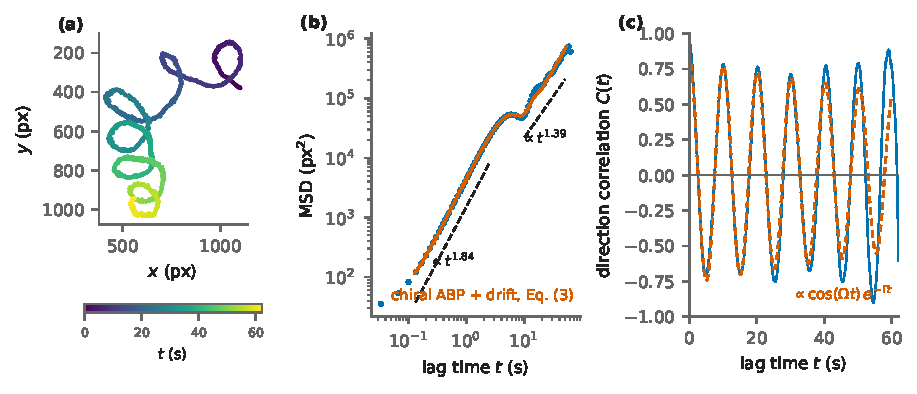
\includegraphics[width=\linewidth]{figures/fig1_single.pdf}
  \caption{A single bug is ballistic at short times; its turning bias then produces a plateau and superdiffusion instead of diffusion. (a)~Trajectory, coloured by time. (b)~Mean square displacement (points) with guides $\propto t^{1.84}$ (ballistic-like, $0.1$--$2.6\,$s) and $\propto t^{1.39}$ ($10$--$52\,$s), and the chiral ABP with drift, Eq.~(\ref{eq:msd}), fitted to the whole curve (orange; $\Omega=0.637\pm0.010\,\mathrm{s^{-1}}$, $v_0=68\,$px/s, $V=15.0\pm0.3\,$px/s, $D_r=0.092\pm0.009\,\mathrm{s^{-1}}$, plus a constant offset for the localisation error). (c)~Direction correlation (blue) with the damped cosine of Eq.~(\ref{eq:corr}) fitted on $0.4$--$20\,$s (orange; $\Omega=0.623\,\mathrm{s^{-1}}$, $\Gamma=0.0057\pm0.0006\,\mathrm{s^{-1}}$, $R^2=0.994$).}
  \label{fig:single}
\end{figure}

Figure~\ref{fig:single}a shows the trajectory of one bug: it traces loops that slowly march across the arena.
The direction correlation (Fig.~\ref{fig:single}c) oscillates with a period of $10.1\,$s, i.e.\ $\Omega=0.623\,\mathrm{s^{-1}}$, and shows no visible decay over the $60\,$s recording ($\Gamma=0.0057\,\mathrm{s^{-1}}$, a decay time of $\approx175\,$s from the fit window $0.4$--$20\,$s), so the circling is phase coherent for much longer than a period.
The MSD (Fig.~\ref{fig:single}b) follows a nearly ballistic law, $\propto t^{1.84}$, for $0.1<t<2.6\,$s, saturates near $5\times10^4\,\mathrm{px^2}$ at half a period, dips at $t\approx10\,$s (one period), and then grows again as $\propto t^{1.39}$.
The ballistic regime is the one expected for an ABP, but the long-time behaviour is not: there is no diffusive regime, because the characteristic time is the circling period $2\pi/\Omega\approx10\,$s set by the turning bias and the long-time growth is faster than diffusive.
Equation~(\ref{eq:msd}) fitted to the entire MSD ($0.13$--$52\,$s, rms deviation $7\%$ on a logarithmic scale) gives $\Omega=0.637\pm0.010\,\mathrm{s^{-1}}$, within $2\%$ of the value from the correlation, a speed $v_0=68\,$px/s, an orbit radius $R=v_0/\Omega\approx106\,$px and a drift $V=15.0\pm0.3\,$px/s.
The drift is not a free parameter in disguise: the orbit centre, estimated as the position averaged over one period, moves at $16.0\,$px/s in the trajectory itself.
The superdiffusive exponent is thus the signature of a drifting orbit, $\langle\Delta r^2\rangle\to V^2t^2$ at long times.
A second recording shows the same sequence (ballistic exponent $1.81$ on $0.3$--$3\,$s, a plateau, then growth with exponent $1.57$ on $12$--$50\,$s; $\Omega=0.53\,\mathrm{s^{-1}}$) with a weaker and faster decaying correlation ($a_1=0.11$, $\Gamma=0.073\,\mathrm{s^{-1}}$).

The model does not reproduce everything.
The decoherence rate needed by the MSD, $D_r=0.092\pm0.009\,\mathrm{s^{-1}}$, is sixteen times larger than the decay rate of the correlation, $\Gamma=0.0057\,\mathrm{s^{-1}}$, which is itself a fit over $0.4$--$20\,$s.
The loops in Fig.~\ref{fig:single}a become smaller with time, so $v_0$ or $\Omega$ is not constant, and a constant-parameter model will absorb such slow changes into an effective $D_r$; we therefore regard $D_r$ from the MSD as an upper bound, but we have not tested which parameter drifts (for example with the state of the battery).
The cause of the drift of the orbit centre, which Eqs.~(\ref{eq:r})--(\ref{eq:th}) simply assume, is also unknown to us.

Having characterised the single particle, we ask what such a bath does to objects it pushes.
A passive thermal bath cannot spin a gear in a preferred direction, but a bath of persistent particles can: a particle that slides along the saw-tooth edge of a gear is trapped in a concave corner and keeps pushing there, and when the teeth are asymmetric the torques from the two sliding directions do not cancel~\cite{Angelani2009,DiLeonardo2010,Sokolov2010}.
The sense of rotation should then be set by the handedness of the teeth.
We tested this with two gears whose teeth have opposite orientation (Fig.~\ref{fig:spinner}a,b) in a bath of $N=10$ and $N=17$ bugs, tracking the angle $\vartheta(t)$ of the line joining the two painted markers.
In each window of $8\,$s we fit $\vartheta(t)$ linearly; the slope is the window's angular velocity $\omega$ (positive counter-clockwise).

\begin{figure}[tb]
  \centering
  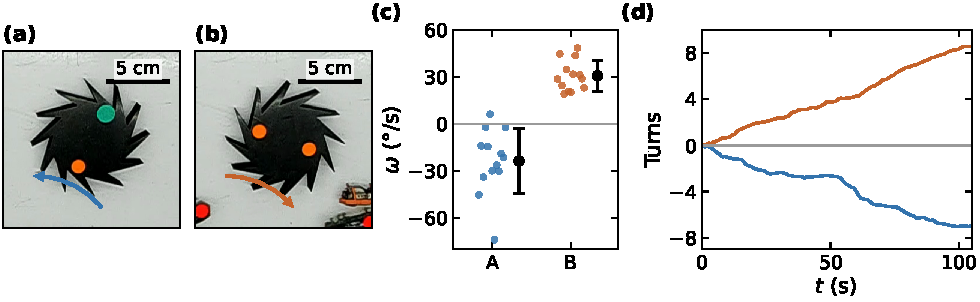
\includegraphics[width=\linewidth]{figures/fig2_spinner.pdf}
  \caption{The handedness of the teeth sets the sense of rotation. (a,b)~The two gears with the measured sense of rotation. (c)~Angular velocity in $8\,$s windows (dots), mean $\pm$ SD (bars); solid: $N=10$ bugs, hatched: $N=17$. (d)~Accumulated rotation in turns (solid: $N=10$, dashed: $N=17$; final values at the right end). The recording with gear~A and 17 bugs stops at $104\,$s, when the gear was replaced by hand.}
  \label{fig:spinner}
\end{figure}

Figure~\ref{fig:spinner} shows that the two gears turn in opposite senses: gear~A clockwise and gear~B counter-clockwise, for both $N$.
Each gear keeps its sense: in $49$ of the $53$ windows the gear turned in the sense of its overall rotation ($8/10$ and $12/13$ for gear~A with $10$ and $17$ bugs; $10/11$ and $19/19$ for gear~B).
With one gear of each handedness, we cannot exclude that other differences between the two objects contribute; the tooth orientation is the difference we designed.
The mean angular velocities are $-39\pm29$ and $-24\pm21\,^\circ$/s for gear~A and $+27\pm20$ and $+25\pm13\,^\circ$/s for gear~B ($N=10$ and $17$; mean $\pm$ SD over windows), which accumulate to between $7$ and $11$ turns over the recordings (Fig.~\ref{fig:spinner}d).
The rotation is irregular: the gear stalls for tens of seconds and restarts (plateaus in the bottom panels), consistent with a torque delivered by discrete, intermittent pushes.
The difference between $N=10$ and $N=17$ is smaller than the window-to-window spread, so we cannot resolve a dependence on the number of particles.
One possibility is that a more crowded gear is partly jammed, since steric interactions are known to reduce rectification at high density by clogging~\cite{Wan2008}; with two densities we cannot test this.

We now turn from rotation to translation.
A straight rod is mirror symmetric along and across its axis, so by symmetry its velocity along the axis must average to zero.
An L-shaped rod has a single mirror axis, the bisector of its arms, which defines a polar direction (from the corner to the opening) along which a net force is allowed, as for the funnels above~\cite{Galajda2007,Wan2008}.
We therefore measured the velocity of the centre of mass $\mathbf R$ in the frame of the rod,
\begin{equation}
  v_\parallel=\dot{\mathbf R}\cdot\ee_b ,
  \label{eq:vpar}
\end{equation}
where $\ee_b$ is the unit vector along the rod's axis (from the corner to the opening for the L; the long axis, with arbitrary sign, for the straight rod), obtained by fitting the rod's outline in every frame.
Both rods were in a bath of 17 bugs and have the same projected area ($11.3\times10^3\,\mathrm{px^2}$).
We compute $\dot{\mathbf R}$ over $1\,$s, and average $v_\parallel$ of Eq.~(\ref{eq:vpar}) over windows of $8\,$s that contain no hand ($10$ windows for the L, $8$ for the straight rod).

\begin{figure}[tb]
  \centering
  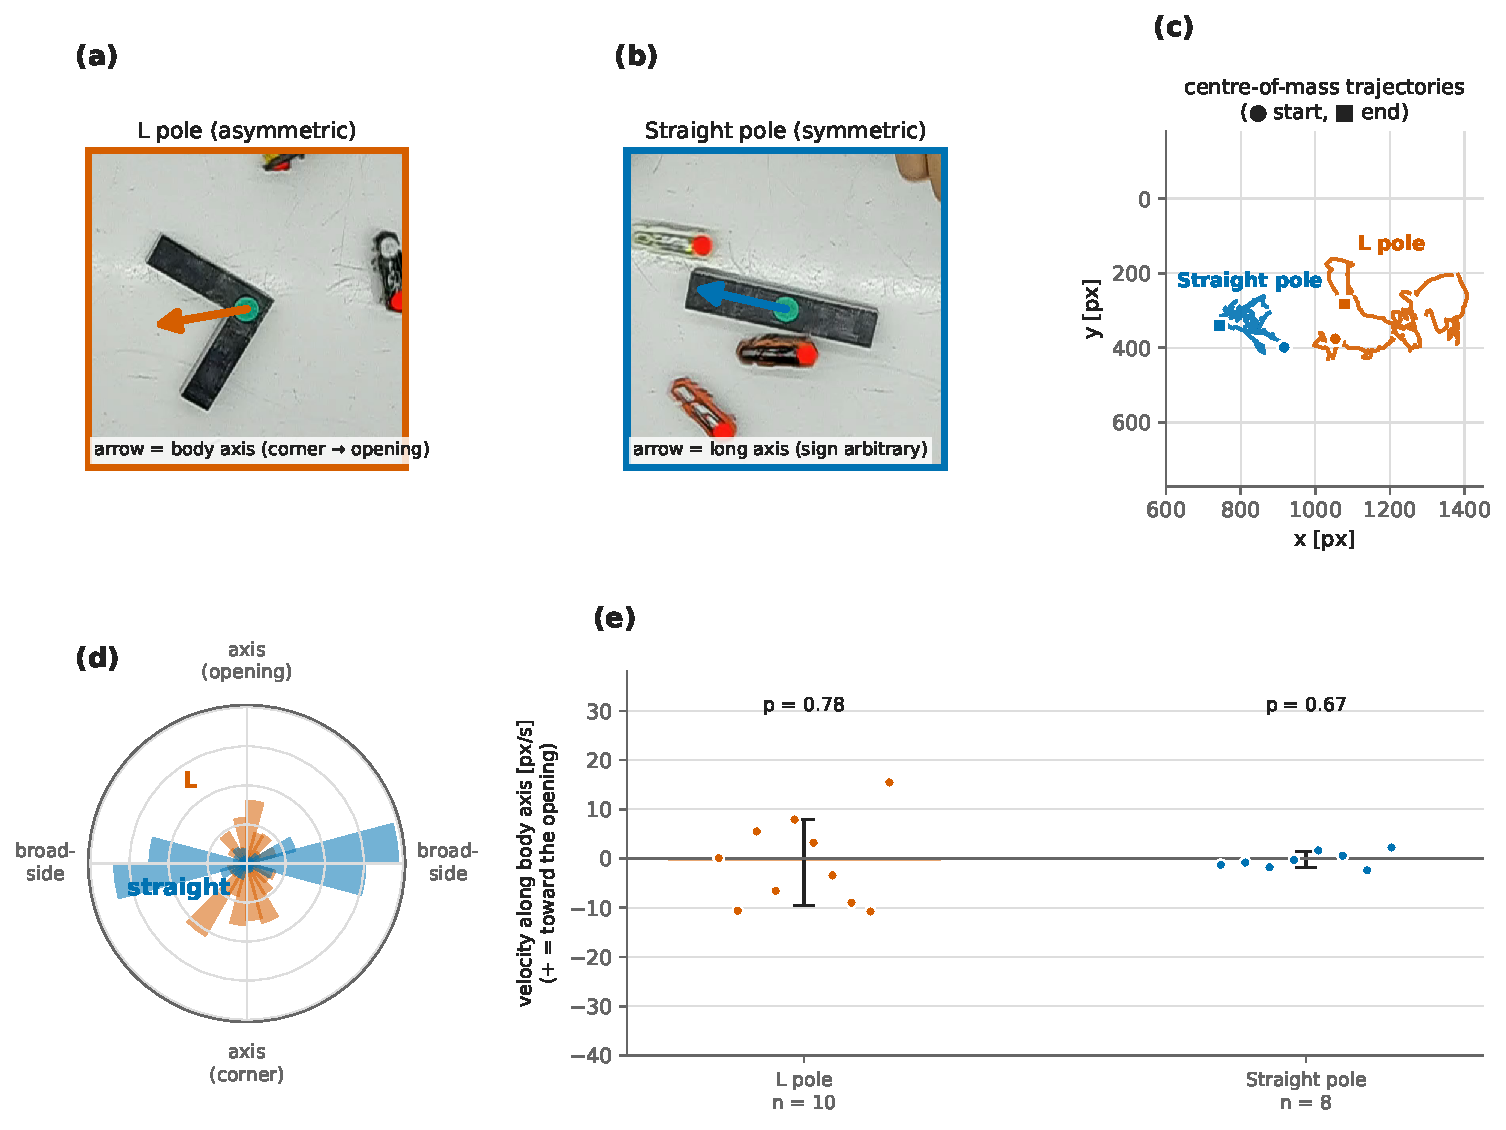
\includegraphics[width=\linewidth]{figures/fig3_poles.pdf}
  \caption{Translation of an L-shaped and a straight rod in a bath of 17 bugs. (a,b)~The rods with their body axes (arrows). (c)~Trajectories of their centres of mass (circle: start, square: end). (d)~Direction of motion in the rod's frame, speed weighted, all hand-free data (orange: L, blue: straight). (e)~Velocity along the body axis in $8\,$s windows (dots), mean $\pm$ SD (bars) and $p$ of a two-sided $t$-test against zero; for the straight rod the sign of the axis is arbitrary (negative in 5 of 8 windows; L: 5 of 10 toward the corner).}
  \label{fig:poles}
\end{figure}

The straight rod moves mostly broadside, perpendicular to its length, and equally in both senses (Fig.~\ref{fig:poles}d): a bug that hits the long side pushes it along the normal to that side, and there are no net pushes along the axis, $\langle v_\parallel\rangle=-0.3\pm1.6\,$px/s (mean $\pm$ SD over windows; $t$-test against zero $p=0.67$).
This is the control: it shows that the measurement has no spurious bias at the level of $\approx1.5\,$px/s (the $95\%$ confidence interval of this mean).
The L-shaped rod moves differently.
It is faster, $20.6$ against $13.6\,$px/s in the mean over windows (Mann--Whitney $p=2\times10^{-4}$), and wanders over a larger part of the arena (Fig.~\ref{fig:poles}c).
A plausible, untested reason is that bugs trapped in its concave corner push it persistently.
Its direction, however, is not established.
The distribution of directions pooled over all frames leans toward the corner (Fig.~\ref{fig:poles}d), but the window averages $\langle v_\parallel\rangle=-0.8\pm8.8\,$px/s are positive in 5 and negative in 5 of the 10 windows ($p=0.78$), and the directions of the window-averaged velocities in the rod's frame are not clustered along any axis (Rayleigh test, $p=0.95$).
The pooled lean therefore comes from a few fast runs and does not persist from window to window.
With $10$ windows our $95\%$ confidence interval for the mean is $-0.8\pm6.3\,$px/s, so a preferred velocity along the axis larger than about $7\,$px/s, one third of the mean speed, is excluded; a smaller one is not.
We treat consecutive windows as independent, which is an approximation.

Finally, we turn from single objects to collective behaviour of the bugs themselves.
We placed $N=5$, 7, 10, 15 and 20 bugs in a circular arena \todo{arena diameter in cm, ring material, recording duration for each $N$} and ask whether they cluster or flock as $N$ increases.
A natural observable is the number fluctuation.
Dividing the arena into sub-regions and counting the number $N$ of bugs in a sub-region at each time, the number fluctuation is
\begin{equation}
  \Delta N=\sqrt{\langle N^2\rangle-\langle N\rangle^2}\;\propto\;\langle N\rangle^{\alpha}.
  \label{eq:gnf}
\end{equation}
For uncorrelated particles (an ideal gas) $N$ is Poisson distributed, so $\Delta N^2=\langle N\rangle$ and $\alpha=1/2$ whatever the size of the sub-region.
Clustering enhances $\Delta N$: if clusters of $s$ bugs act as independent units, $\Delta N^2=\langle N\rangle\langle s^2\rangle/\langle s\rangle$ for sub-regions much larger than a cluster, so that $\Delta N^2/\langle N\rangle$ exceeds one by an amount set by the cluster size.
In orientationally ordered active systems $\Delta N$ grows faster than $\langle N\rangle^{1/2}$ ($\alpha>1/2$, ``giant'' number fluctuations), as seen in vibrated rods~\cite{Narayan2007} and in vibrated polar disks~\cite{Deseigne2010}.
Because the total number of bugs is fixed, $\Delta N$ vanishes when the sub-region is the whole arena, so Eq.~(\ref{eq:gnf}) can hold only for sub-regions much smaller than the arena.
\todo{Method: how bug positions were obtained for the flocking videos, the sub-region shape and the range of sizes used, and how $\alpha$ was fitted (with uncertainty, using windows as for the other experiments).}

\todo{Results, to be written after the analysis: (i) Fig.~\ref{fig:flock}a, example frames at the different $N$, noting jammed clusters at the wall; (ii) Fig.~\ref{fig:flock}b, $\Delta N$ against $\langle N\rangle$ on logarithmic axes, with assisting lines $\propto\langle N\rangle^{1/2}$ and $\propto\langle N\rangle$ instead of a legend, one curve per bug number; (iii) Fig.~\ref{fig:flock}c, the exponent $\alpha$ (or $\Delta N^2/\langle N\rangle$) against $N$. Discuss what the exponent says about clustering and flocking at each $N$ (Vicsek-like alignment would give $\alpha>1/2$), the cluster size implied by the box size at which $\Delta N^2/\langle N\rangle$ saturates, and any discrepancy from the ideal-gas value.}

\begin{figure}[tb]
  \centering
  \fbox{\parbox[c][6.5cm][c]{0.94\linewidth}{\centering \todo{Figure~4: flocking. (a) example frames for $N=5,7,10,15,20$; (b) $\Delta N$ vs $\langle N\rangle$ (log--log, guides $\propto\langle N\rangle^{1/2}$ and $\propto\langle N\rangle$); (c) exponent $\alpha$ vs $N$.}}}
  \caption{\todo{Caption of the flocking figure: define every panel, the sub-region used, and the uncertainty shown.}}
  \label{fig:flock}
\end{figure}

In summary, the persistent motion of a bath of self-propelled robots is rectified by the symmetry of the objects it pushes.
Gears with opposite tooth orientation turn in opposite senses, each steadily (in $49$ of $53$ windows), at tens of degrees per second and without a resolvable dependence on the number of bugs between 10 and 17.
A symmetric rod shows no net motion along its axis, as symmetry requires, while an L-shaped rod is faster but we find no significant preferred direction; deciding this would need more or longer recordings.
A single bug is ballistic for about $2.6\,$s as an active Brownian particle, and its weak turning bias and drift explain why its mean square displacement shows a plateau and superdiffusion rather than diffusion.
Two discrepancies remain: the decoherence rate of the orbit differs by a factor of sixteen between the MSD and the correlation, and the drift of the orbit centre is not explained.
\todo{one sentence on flocking}

\bibliography{references}

\end{document}
